\documentclass[UTF8,zihao=-4]{ctexart}
\usepackage[a4paper,margin=2.2cm]{geometry}
\usepackage{amsmath,amssymb}
\usepackage{booktabs,array}
\usepackage{longtable}
\usepackage{graphicx}
\usepackage[hidelinks]{hyperref}
\usepackage{url}

\setlength{\parindent}{2em}

\title{补充材料：重叠窗口拓扑扫描的有限样本校准边界}
\author{}
\date{}

\begin{document}
\maketitle

正文引用本补充材料时按 S1--S5 编号。所有数值与正文及冻结的 canonical 汇总文件一致。

\section*{S1 完整 112 行零假设结果}

下表给出 28 个唯一零假设配置 $\times$ 2 表示 $\times$ 2 方法共 112 个逐格评价单元的
拒绝率（每格 $n=2500$）、95\% Wilson 区间（无连续性修正）与四类校准状态。
列含义：DGP 为数据生成过程；$\rho$ 为原序列依赖；$s$ 为步长；$T$、$M$ 为观测长度与窗口数；
分类取实用校准 / 实质保守 / 实质反保守 / 未定。本表的分类列即正文第 5.2 节所称的
完整状态转换清单。

\begingroup
\footnotesize
\begin{longtable}{llrlrlrrc c}
\toprule
DGP & $\rho$ & $s$ & $T$ & $M$ & 表示 & 方法 & 拒绝率 & 95\% Wilson & 分类\\
\midrule
\endhead
N-AR & 0.8 & 64 & 12288 & 192 & BPI & M0 & 0.0524 & [0.0443,0.0618] & 实用校准\\
N-AR & 0.8 & 64 & 12288 & 192 & BPI & M1 & 0.0276 & [0.0219,0.0348] & 实质保守\\
N-AR & 0.8 & 64 & 12288 & 192 & MOMENTS & M0 & 0.0432 & [0.0359,0.0519] & 实用校准\\
N-AR & 0.8 & 64 & 12288 & 192 & MOMENTS & M1 & 0.0216 & [0.0166,0.0281] & 实质保守\\
N-AR & 0 & 32 & 6176 & 192 & BPI & M0 & 0.3044 & [0.2867,0.3227] & 实质反保守\\
N-AR & 0 & 32 & 6176 & 192 & BPI & M1 & 0.0492 & [0.0414,0.0584] & 实用校准\\
N-AR & 0 & 32 & 6176 & 192 & MOMENTS & M0 & 0.4376 & [0.4183,0.4571] & 实质反保守\\
N-AR & 0 & 32 & 6176 & 192 & MOMENTS & M1 & 0.0404 & [0.0334,0.0488] & 未定\\
N-CIRCLE & 0 & 8 & 1592 & 192 & BPI & M0 & 0.8816 & [0.8683,0.8937] & 实质反保守\\
N-CIRCLE & 0 & 8 & 1592 & 192 & BPI & M1 & 0.0436 & [0.0363,0.0523] & 实用校准\\
N-CIRCLE & 0 & 8 & 1592 & 192 & MOMENTS & M0 & 0.9988 & [0.9965,0.9996] & 实质反保守\\
N-CIRCLE & 0 & 8 & 1592 & 192 & MOMENTS & M1 & 0.0700 & [0.0606,0.0807] & 未定\\
N-AR & 0 & 8 & 1592 & 192 & BPI & M0 & 0.9712 & [0.9639,0.9771] & 实质反保守\\
N-AR & 0 & 8 & 1592 & 192 & BPI & M1 & 0.0808 & [0.0707,0.0921] & 实质反保守\\
N-AR & 0 & 8 & 1592 & 192 & MOMENTS & M0 & 0.9976 & [0.9948,0.9989] & 实质反保守\\
N-AR & 0 & 8 & 1592 & 192 & MOMENTS & M1 & 0.0712 & [0.0618,0.0820] & 未定\\
N-CIRCLE & 0.8 & 8 & 1592 & 192 & BPI & M0 & 0.9384 & [0.9283,0.9472] & 实质反保守\\
N-CIRCLE & 0.8 & 8 & 1592 & 192 & BPI & M1 & 0.0496 & [0.0418,0.0588] & 实用校准\\
N-CIRCLE & 0.8 & 8 & 1592 & 192 & MOMENTS & M0 & 0.9968 & [0.9937,0.9984] & 实质反保守\\
N-CIRCLE & 0.8 & 8 & 1592 & 192 & MOMENTS & M1 & 0.0792 & [0.0692,0.0904] & 实质反保守\\
N-AR & 0 & 64 & 3120 & 48 & BPI & M0 & 0.0608 & [0.0521,0.0709] & 未定\\
N-AR & 0 & 64 & 3120 & 48 & BPI & M1 & 0.0088 & [0.0058,0.0133] & 实质保守\\
N-AR & 0 & 64 & 3120 & 48 & MOMENTS & M0 & 0.0584 & [0.0499,0.0683] & 未定\\
N-AR & 0 & 64 & 3120 & 48 & MOMENTS & M1 & 0.0020 & [0.0009,0.0047] & 实质保守\\
N-CIRCLE & 0 & 64 & 12288 & 192 & BPI & M0 & 0.0528 & [0.0447,0.0623] & 实用校准\\
N-CIRCLE & 0 & 64 & 12288 & 192 & BPI & M1 & 0.0244 & [0.0190,0.0312] & 实质保守\\
N-CIRCLE & 0 & 64 & 12288 & 192 & MOMENTS & M0 & 0.0532 & [0.0451,0.0627] & 实用校准\\
N-CIRCLE & 0 & 64 & 12288 & 192 & MOMENTS & M1 & 0.0228 & [0.0176,0.0294] & 实质保守\\
N-AR & 0.8 & 64 & 3120 & 48 & BPI & M0 & 0.0548 & [0.0465,0.0644] & 实用校准\\
N-AR & 0.8 & 64 & 3120 & 48 & BPI & M1 & 0.0108 & [0.0074,0.0157] & 实质保守\\
N-AR & 0.8 & 64 & 3120 & 48 & MOMENTS & M0 & 0.0492 & [0.0414,0.0584] & 实用校准\\
N-AR & 0.8 & 64 & 3120 & 48 & MOMENTS & M1 & 0.0056 & [0.0033,0.0094] & 实质保守\\
N-CIRCLE & 0.8 & 64 & 3120 & 48 & BPI & M0 & 0.0552 & [0.0469,0.0649] & 实用校准\\
N-CIRCLE & 0.8 & 64 & 3120 & 48 & BPI & M1 & 0.0056 & [0.0033,0.0094] & 实质保守\\
N-CIRCLE & 0.8 & 64 & 3120 & 48 & MOMENTS & M0 & 0.0616 & [0.0528,0.0717] & 未定\\
N-CIRCLE & 0.8 & 64 & 3120 & 48 & MOMENTS & M1 & 0.0032 & [0.0016,0.0063] & 实质保守\\
N-AR & 0.8 & 8 & 3120 & 383 & BPI & M0 & 0.9480 & [0.9386,0.9560] & 实质反保守\\
N-AR & 0.8 & 8 & 3120 & 383 & BPI & M1 & 0.1180 & [0.1059,0.1312] & 实质反保守\\
N-AR & 0.8 & 8 & 3120 & 383 & MOMENTS & M0 & 0.9912 & [0.9867,0.9942] & 实质反保守\\
N-AR & 0.8 & 8 & 3120 & 383 & MOMENTS & M1 & 0.1064 & [0.0949,0.1191] & 实质反保守\\
N-CIRCLE & 0 & 64 & 3120 & 48 & BPI & M0 & 0.0472 & [0.0396,0.0562] & 实用校准\\
N-CIRCLE & 0 & 64 & 3120 & 48 & BPI & M1 & 0.0060 & [0.0036,0.0099] & 实质保守\\
N-CIRCLE & 0 & 64 & 3120 & 48 & MOMENTS & M0 & 0.0520 & [0.0440,0.0614] & 实用校准\\
N-CIRCLE & 0 & 64 & 3120 & 48 & MOMENTS & M1 & 0.0024 & [0.0011,0.0052] & 实质保守\\
N-CIRCLE & 0 & 16 & 3120 & 192 & BPI & M0 & 0.4384 & [0.4191,0.4579] & 实质反保守\\
N-CIRCLE & 0 & 16 & 3120 & 192 & BPI & M1 & 0.0480 & [0.0403,0.0571] & 实用校准\\
N-CIRCLE & 0 & 16 & 3120 & 192 & MOMENTS & M0 & 0.9376 & [0.9274,0.9464] & 实质反保守\\
N-CIRCLE & 0 & 16 & 3120 & 192 & MOMENTS & M1 & 0.0760 & [0.0663,0.0871] & 实质反保守\\
N-AR & 0.8 & 32 & 3120 & 96 & BPI & M0 & 0.2668 & [0.2498,0.2845] & 实质反保守\\
N-AR & 0.8 & 32 & 3120 & 96 & BPI & M1 & 0.0352 & [0.0287,0.0432] & 未定\\
N-AR & 0.8 & 32 & 3120 & 96 & MOMENTS & M0 & 0.3336 & [0.3154,0.3523] & 实质反保守\\
N-AR & 0.8 & 32 & 3120 & 96 & MOMENTS & M1 & 0.0228 & [0.0176,0.0294] & 实质保守\\
N-AR & 0 & 16 & 3120 & 192 & BPI & M0 & 0.7356 & [0.7180,0.7525] & 实质反保守\\
N-AR & 0 & 16 & 3120 & 192 & BPI & M1 & 0.0672 & [0.0580,0.0777] & 未定\\
N-AR & 0 & 16 & 3120 & 192 & MOMENTS & M0 & 0.9136 & [0.9019,0.9240] & 实质反保守\\
N-AR & 0 & 16 & 3120 & 192 & MOMENTS & M1 & 0.0680 & [0.0588,0.0785] & 未定\\
N-CIRCLE & 0.8 & 32 & 6176 & 192 & BPI & M0 & 0.1556 & [0.1419,0.1703] & 实质反保守\\
N-CIRCLE & 0.8 & 32 & 6176 & 192 & BPI & M1 & 0.0280 & [0.0222,0.0352] & 未定\\
N-CIRCLE & 0.8 & 32 & 6176 & 192 & MOMENTS & M0 & 0.4560 & [0.4366,0.4756] & 实质反保守\\
N-CIRCLE & 0.8 & 32 & 6176 & 192 & MOMENTS & M1 & 0.0472 & [0.0396,0.0562] & 实用校准\\
N-CIRCLE & 0 & 32 & 6176 & 192 & BPI & M0 & 0.1088 & [0.0972,0.1216] & 实质反保守\\
N-CIRCLE & 0 & 32 & 6176 & 192 & BPI & M1 & 0.0284 & [0.0226,0.0357] & 未定\\
N-CIRCLE & 0 & 32 & 6176 & 192 & MOMENTS & M0 & 0.4984 & [0.4788,0.5180] & 实质反保守\\
N-CIRCLE & 0 & 32 & 6176 & 192 & MOMENTS & M1 & 0.0332 & [0.0269,0.0410] & 未定\\
N-CIRCLE & 0.8 & 32 & 3120 & 96 & BPI & M0 & 0.1584 & [0.1446,0.1732] & 实质反保守\\
N-CIRCLE & 0.8 & 32 & 3120 & 96 & BPI & M1 & 0.0184 & [0.0138,0.0245] & 实质保守\\
N-CIRCLE & 0.8 & 32 & 3120 & 96 & MOMENTS & M0 & 0.4144 & [0.3952,0.4338] & 实质反保守\\
N-CIRCLE & 0.8 & 32 & 3120 & 96 & MOMENTS & M1 & 0.0276 & [0.0219,0.0348] & 实质保守\\
N-AR & 0 & 32 & 3120 & 96 & BPI & M0 & 0.2776 & [0.2604,0.2955] & 实质反保守\\
N-AR & 0 & 32 & 3120 & 96 & BPI & M1 & 0.0288 & [0.0229,0.0361] & 未定\\
N-AR & 0 & 32 & 3120 & 96 & MOMENTS & M0 & 0.4260 & [0.4067,0.4455] & 实质反保守\\
N-AR & 0 & 32 & 3120 & 96 & MOMENTS & M1 & 0.0212 & [0.0162,0.0276] & 实质保守\\
N-AR & 0.8 & 16 & 3120 & 192 & BPI & M0 & 0.6688 & [0.6501,0.6870] & 实质反保守\\
N-AR & 0.8 & 16 & 3120 & 192 & BPI & M1 & 0.0788 & [0.0689,0.0900] & 实质反保守\\
N-AR & 0.8 & 16 & 3120 & 192 & MOMENTS & M0 & 0.7928 & [0.7765,0.8082] & 实质反保守\\
N-AR & 0.8 & 16 & 3120 & 192 & MOMENTS & M1 & 0.0628 & [0.0539,0.0730] & 未定\\
N-CIRCLE & 0 & 8 & 3120 & 383 & BPI & M0 & 0.8900 & [0.8771,0.9017] & 实质反保守\\
N-CIRCLE & 0 & 8 & 3120 & 383 & BPI & M1 & 0.0808 & [0.0707,0.0921] & 实质反保守\\
N-CIRCLE & 0 & 8 & 3120 & 383 & MOMENTS & M0 & 0.9996 & [0.9977,0.9999] & 实质反保守\\
N-CIRCLE & 0 & 8 & 3120 & 383 & MOMENTS & M1 & 0.1320 & [0.1193,0.1458] & 实质反保守\\
N-AR & 0.8 & 8 & 1592 & 192 & BPI & M0 & 0.9324 & [0.9219,0.9416] & 实质反保守\\
N-AR & 0.8 & 8 & 1592 & 192 & BPI & M1 & 0.0892 & [0.0786,0.1010] & 实质反保守\\
N-AR & 0.8 & 8 & 1592 & 192 & MOMENTS & M0 & 0.9816 & [0.9755,0.9862] & 实质反保守\\
N-AR & 0.8 & 8 & 1592 & 192 & MOMENTS & M1 & 0.0676 & [0.0584,0.0781] & 未定\\
N-CIRCLE & 0.8 & 16 & 3120 & 192 & BPI & M0 & 0.5416 & [0.5220,0.5611] & 实质反保守\\
N-CIRCLE & 0.8 & 16 & 3120 & 192 & BPI & M1 & 0.0524 & [0.0443,0.0618] & 实用校准\\
N-CIRCLE & 0.8 & 16 & 3120 & 192 & MOMENTS & M0 & 0.8796 & [0.8663,0.8918] & 实质反保守\\
N-CIRCLE & 0.8 & 16 & 3120 & 192 & MOMENTS & M1 & 0.0848 & [0.0745,0.0964] & 实质反保守\\
N-CIRCLE & 0.8 & 8 & 3120 & 383 & BPI & M0 & 0.9432 & [0.9334,0.9516] & 实质反保守\\
N-CIRCLE & 0.8 & 8 & 3120 & 383 & BPI & M1 & 0.0824 & [0.0723,0.0938] & 实质反保守\\
N-CIRCLE & 0.8 & 8 & 3120 & 383 & MOMENTS & M0 & 0.9964 & [0.9932,0.9981] & 实质反保守\\
N-CIRCLE & 0.8 & 8 & 3120 & 383 & MOMENTS & M1 & 0.1412 & [0.1281,0.1554] & 实质反保守\\
N-CIRCLE & 0.8 & 64 & 12288 & 192 & BPI & M0 & 0.0528 & [0.0447,0.0623] & 实用校准\\
N-CIRCLE & 0.8 & 64 & 12288 & 192 & BPI & M1 & 0.0244 & [0.0190,0.0312] & 实质保守\\
N-CIRCLE & 0.8 & 64 & 12288 & 192 & MOMENTS & M0 & 0.0516 & [0.0436,0.0610] & 实用校准\\
N-CIRCLE & 0.8 & 64 & 12288 & 192 & MOMENTS & M1 & 0.0236 & [0.0183,0.0303] & 实质保守\\
N-AR & 0 & 64 & 12288 & 192 & BPI & M0 & 0.0504 & [0.0425,0.0597] & 实用校准\\
N-AR & 0 & 64 & 12288 & 192 & BPI & M1 & 0.0224 & [0.0173,0.0290] & 实质保守\\
N-AR & 0 & 64 & 12288 & 192 & MOMENTS & M0 & 0.0492 & [0.0414,0.0584] & 实用校准\\
N-AR & 0 & 64 & 12288 & 192 & MOMENTS & M1 & 0.0192 & [0.0145,0.0254] & 实质保守\\
N-AR & 0 & 8 & 3120 & 383 & BPI & M0 & 0.9756 & [0.9688,0.9810] & 实质反保守\\
N-AR & 0 & 8 & 3120 & 383 & BPI & M1 & 0.1136 & [0.1017,0.1266] & 实质反保守\\
N-AR & 0 & 8 & 3120 & 383 & MOMENTS & M0 & 0.9984 & [0.9959,0.9994] & 实质反保守\\
N-AR & 0 & 8 & 3120 & 383 & MOMENTS & M1 & 0.1184 & [0.1063,0.1317] & 实质反保守\\
N-AR & 0.8 & 32 & 6176 & 192 & BPI & M0 & 0.2640 & [0.2471,0.2816] & 实质反保守\\
N-AR & 0.8 & 32 & 6176 & 192 & BPI & M1 & 0.0408 & [0.0337,0.0493] & 未定\\
N-AR & 0.8 & 32 & 6176 & 192 & MOMENTS & M0 & 0.3440 & [0.3256,0.3628] & 实质反保守\\
N-AR & 0.8 & 32 & 6176 & 192 & MOMENTS & M1 & 0.0312 & [0.0251,0.0388] & 未定\\
N-CIRCLE & 0 & 32 & 3120 & 96 & BPI & M0 & 0.1200 & [0.1078,0.1333] & 实质反保守\\
N-CIRCLE & 0 & 32 & 3120 & 96 & BPI & M1 & 0.0188 & [0.0142,0.0249] & 实质保守\\
N-CIRCLE & 0 & 32 & 3120 & 96 & MOMENTS & M0 & 0.4820 & [0.4625,0.5016] & 实质反保守\\
N-CIRCLE & 0 & 32 & 3120 & 96 & MOMENTS & M1 & 0.0164 & [0.0121,0.0222] & 实质保守\\
\bottomrule
\end{longtable}
\endgroup

\section*{S2 完整 16 行备择结果}

下表给出两个场景 $\times$ 4 条件 $\times$ 2 表示共 16 个“条件--表示”单元的
尺寸校正功效、归一化定位误差、联合成功率与名义功效（每格 $n=1600$，临界秩 2376）。
列含义：$\rho$ 为原序列依赖；$s$ 为步长；$J_0$、$J_1$ 分别为 M0、M1 的联合成功率；
$\beta_0$、$\beta_1$ 分别为 M0、M1 的名义功效。

\begingroup
\footnotesize
\begin{longtable}{llrlrrrrrr}
\toprule
场景 & $\rho$ & $s$ & 表示 & 尺寸校正功效 & nMAE & $J_0$ & $J_1$ & $\beta_0$ & $\beta_1$\\
\midrule
\endhead
形状变化 & 0 & 64 & BPI & 1.00000 & 0.00001 & 0.9988 & 0.9988 & 1.0000 & 1.0000\\
形状变化 & 0 & 64 & MOMENTS & 0.07125 & 0.21158 & 0.0006 & 0.0006 & 0.0531 & 0.0206\\
均值平移 & 0 & 64 & BPI & 0.05312 & 0.20918 & 0.0000 & 0.0000 & 0.0537 & 0.0225\\
均值平移 & 0 & 64 & MOMENTS & 1.00000 & 0.00003 & 0.9944 & 0.9944 & 1.0000 & 1.0000\\
形状变化 & 0.8 & 16 & BPI & 1.00000 & 0.00772 & 0.9912 & 0.9912 & 1.0000 & 1.0000\\
形状变化 & 0.8 & 16 & MOMENTS & 0.04562 & 0.20186 & 0.0350 & 0.0019 & 0.9294 & 0.0825\\
均值平移 & 0.8 & 64 & BPI & 0.04688 & 0.21402 & 0.0006 & 0.0006 & 0.0419 & 0.0187\\
均值平移 & 0.8 & 64 & MOMENTS & 1.00000 & 0.00132 & 0.8119 & 0.8119 & 1.0000 & 1.0000\\
均值平移 & 0 & 16 & BPI & 0.05437 & 0.18659 & 0.0219 & 0.0037 & 0.4437 & 0.0406\\
均值平移 & 0 & 16 & MOMENTS & 1.00000 & 0.00284 & 0.9988 & 0.9988 & 1.0000 & 1.0000\\
均值平移 & 0.8 & 16 & BPI & 0.06062 & 0.20040 & 0.0125 & 0.0000 & 0.5819 & 0.0512\\
均值平移 & 0.8 & 16 & MOMENTS & 1.00000 & 0.00902 & 0.8156 & 0.8156 & 1.0000 & 1.0000\\
形状变化 & 0.8 & 64 & BPI & 1.00000 & 0.00035 & 0.9456 & 0.9456 & 1.0000 & 1.0000\\
形状变化 & 0.8 & 64 & MOMENTS & 0.06688 & 0.18595 & 0.0000 & 0.0000 & 0.0981 & 0.0413\\
形状变化 & 0 & 16 & BPI & 1.00000 & 0.00828 & 1.0000 & 1.0000 & 1.0000 & 1.0000\\
形状变化 & 0 & 16 & MOMENTS & 0.06438 & 0.20720 & 0.0219 & 0.0013 & 0.9500 & 0.0731\\
\bottomrule
\end{longtable}
\endgroup

\section*{S3 主对比与表示差自助法的完整规格}

\textbf{主对比 P1--P3}：使用 10{,}000 次按数据生成过程分层的整簇自助法；同一主重复编号下
的全部相关条件、表示和方法随簇共同重采样。单侧自助 $p$ 值按加一规则
$p=(1+\#\{\text{尾部}\})/10001$ 计算，三个单侧 $p$ 值经 Holm step-down 校正。
边际 95\% 区间为最近秩（nearest-rank）分位数定义的 basic bootstrap interval。

\textbf{表示差 $\Delta$}：通过两层整簇自助法估计，每层 2000 次。重采样单位为主复制：
零假设层按 N-CIRCLE 主复制整簇重采样以重算经验临界值，备择层按备择主复制整簇重采样以重算功效；
两层分别独立重采样。BPI 与 MOMENTS 使用同一重采样索引成对移动；四个 $(\rho,s)$ 条件
在每个场景内先计算各自的 BPI 减 MOMENTS 功效差，再等权平均得到场景差。
区间采用最近秩定义的 2000 次百分位区间（$2.5\%$ 与 $97.5\%$ 分位数）。

\section*{S4 完整 16$\times$4 热图}

图~\ref{fig:s1}给出 16 个条件（DGP$\times\rho\times s$）$\times$ 4 列
（BPI/M0、BPI/M1、MOMENTS/M0、MOMENTS/M1）的完整逐格 I 类错误率，两个面板分别对应
fixed-$M$ 与 fixed-$T$。色标 $[0,1]$，格内标注四位小数。

\begin{figure}[ht]
\centering
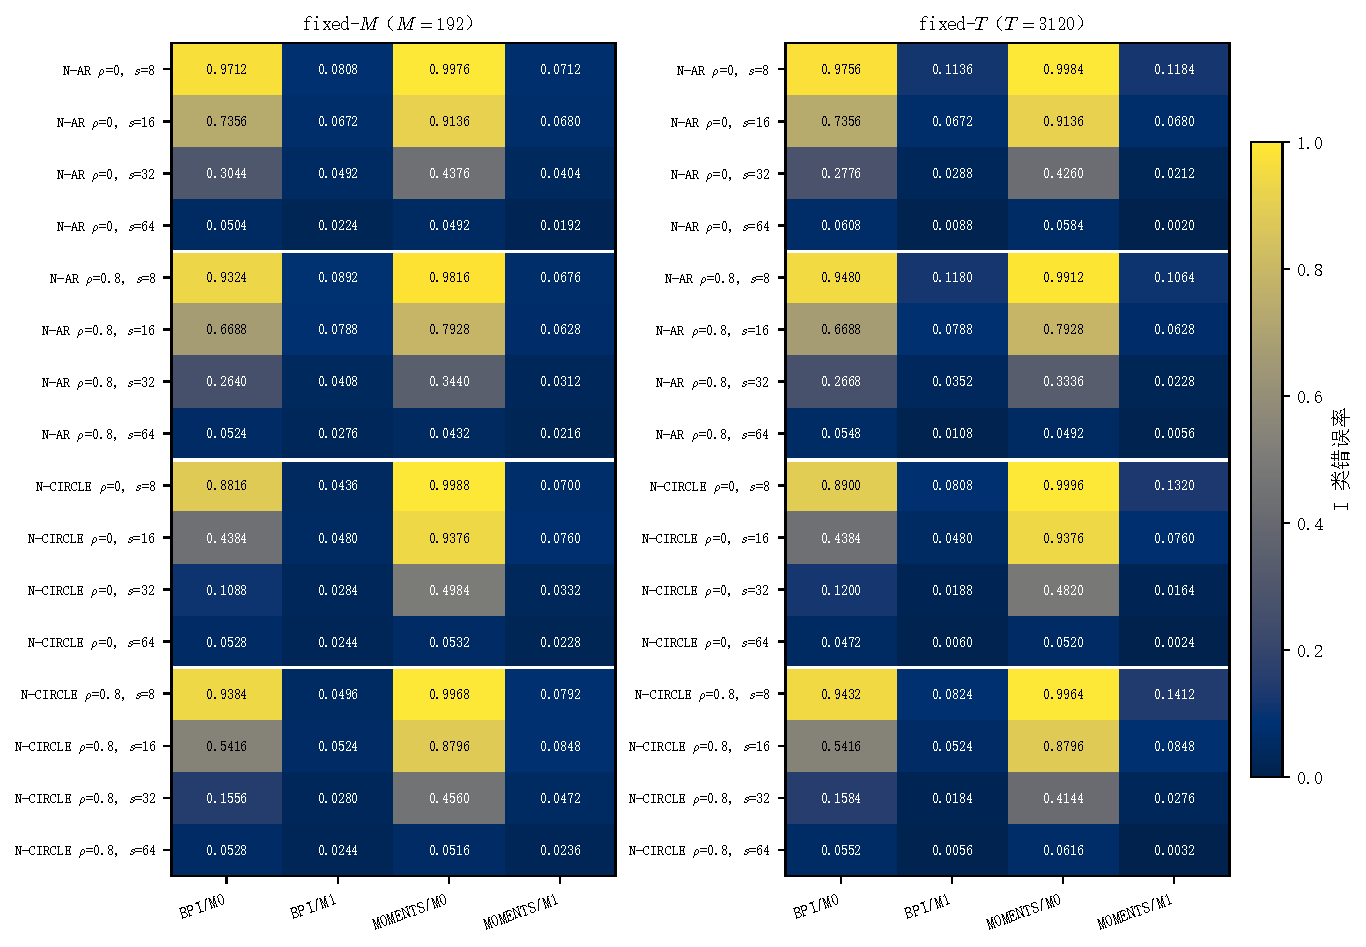
\includegraphics[width=0.95\textwidth]{../../artifacts/figures/FigureS1_H0_16x4_heatmap.pdf}
\caption{完整 16$\times$4 逐格 I 类错误率热图。两面板分别为 fixed-$M$（$M=192$）与
fixed-$T$（$T=3120$）；16 行按 DGP$\times\rho\times s$ 排列，4 列为
BPI/M0、BPI/M1、MOMENTS/M0、MOMENTS/M1。}\label{fig:s1}
\end{figure}

\section*{S5 代码与数据可用性}

复现本文结果的代码、配置、种子清单、完整逐格数据与全部生成脚本由仓库提供：

\begin{itemize}
\item 代码仓库：\url{https://github.com/dw0911/owtda-calibration}
\item 本稿对应 git 标签 \texttt{v1.2.0-paper}
\item 全部合成数据由该版本代码与固定随机种子生成；独立数据 DOI 尚在建立中，未作为已提供材料列出
\end{itemize}

\end{document}
